\subsection{Impact of Simple Scheduling Strategies}
\label{sec3.2-0}

In this section, we introduce a simple segment-based balancing method based on historical records and greedy strategy, which move segments periodically to rebalance the throughput of block servers. Moreover, the influence of different parameters on the scheduling results will be analyzed.

\subsubsection{Introduction to Simple Scheduling Strategies} 
\label{sec3.2-1}

We first define a \textit{simple greedy strategy}, which performs a round of schedule at a specified time interval (to be specified by the administrator). When the time to schedule arrives, the scheduler will calculate the historical average on every segment over a period of time. Then, the scheduler will traverse segments by historical records from high to low. The scheduler will move the segment to the block server which has the lowest throughput. Obviously, schedule frequency and the time length of historical record will make an impact on the schedule result.

In the sections below, we will discuss the impact of several parameters (e.g. knowledge of future throughput, proportion of scheduling segments). All these topics will be discussed on the \textit{simple greedy strategy} as an example.


\subsubsection{Impact of Greedy Algorithm}
\label{sec3.2-2}

We simulate simple greedy algorithm on different clusters. We can find that simple greedy strategy can reduce the variance in some degree, but there's still some distance to the upper limit (Table \ref{table3.2-1}). What's worse, sometimes, negative optimizations may occur (Figure \ref{fig3.2-1}). The reason is that average of historical records can not describe the pattern of the cluster properly. 

\begin{table}[ht]
    \footnotesize
    \centering
    \begin{tabular}{c|c|c|c|c}
         Cluster & Type& No Schedule & Greedy & Future\\
         AY306L & ESSD & 2.13E+18 & 6.51E+17 & 5.36E+17\\
         AY251Z & ESSD & 7.68E+17 & 5.53E+17 & 1.99E+17\\
         AY272T & SSD & 6.87E+17 & 1.10E+17 & 3.02E+16\\
         AY306O & Efficient & 3.08E+17 & 1.14E+17 & 3.29E+06\\
         AY336D & Efficient & 7.27E+17 & 1.12E+17 & 3.35E+06\\
         AY272M & Efficient & 2.97E+17 & 7.75E+16 & 3.52E+06\\
    \end{tabular}
    \caption{Median of cluster variance}
    \label{table3.2-1}
\end{table}

\begin{figure}[ht]
    \centering
    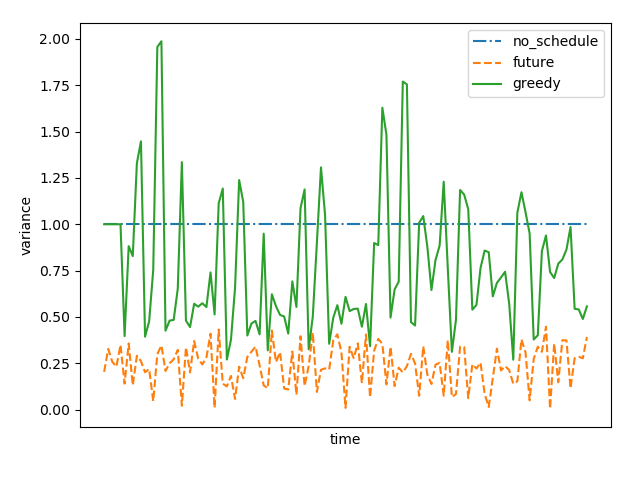
\includegraphics[width=0.4\textwidth]{Figure-3.2/Figure_1-1.png}
    \caption{Result of Simple Greedy Strategy on AY251Z}
    \label{fig3.2-1}
\end{figure}

For example, I/O pattern of many segments is periodic. In cluster AY251Z, the I/O pattern of a device, which has 16 segments and accounts for 9.2\% flow of the whole cluster, is in a cycle of 20 minutes. However, Figure \ref{fig3.2-2} indicates that these segments are in busy only in a short period of the cycle. If the observation range of history is too low, prediction will differ greatly from the actual state. However, if we raise the observation range, in some segments, local characteristics will be missed, though the periodic problem may be solved. As a result, average of historical records can not describe the pattern of the cluster properly. To improve the schedule result, detailed I/O pattern should be extracted for scheduling.


\begin{figure}[ht]
    \centering
    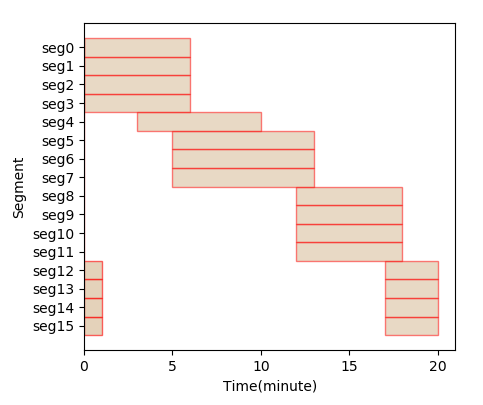
\includegraphics[width=0.4\textwidth]{Figure-3.2/Figure_2.png}
    \caption{Busy Time of Segments in a Certain Device}
    \label{fig3.2-2}
\end{figure}


\subsubsection{Impact of Knowledge of Future Throughput}
\label{sec3.2-3}

Scheduling effect not only depends on strategy itself, but also depends on the schedulability of the cluster. If we can know the future throughput of each segment, the scheduling effect will be improved. Hence, we can analyze the best case of greedy algorithms. We can use the following method to attempt to reach an approximate upper bound for any greedy schedule strategy. In the \textit{simple greedy strategy}, we pretend to know the future throughput of each segment, and execute scheduling with the future throughput. Besides, schedule should be frequent enough, or we will deviate from upper bound.

Table \ref{table3.2-1} shows the initial state and the approximate upper bound of any greedy algorithm. Note that, there is little potential for ESSD clusters to improve, while SSD clusters and efficient clusters have great potential to improve. As was stated in section \ref{sec3.1-3}, ESSD cloud disks have better performance and allow higher throughput. Thus, users are more likely to read and write more to the disk and the smallest unit of scheduling will be larger. This makes scheduling algorithm less effective on clusters with higher performance.


\subsubsection{Impact of Proportion of Segments to Schedule}
\label{sec3.2-4}

According to the 80/20 rule, we have a reason to believe that few segments contributes most to the variance of the entire cluster. Hence, we define a \textit{partial greedy strategy}, which only replace segments with the most throughput in each round of schedule. Evidently, the proportion of segments to schedule each time will also make an impact on the schedule result. Figure \ref{fig3.2-3} shows the relation between variance and the schedule proportion of \textit{partial greedy strategy}. Schedule interval and observation length of history are both 5 minutes.

\begin{figure}[ht]
    \centering
    \subfigure[AY336D]{
        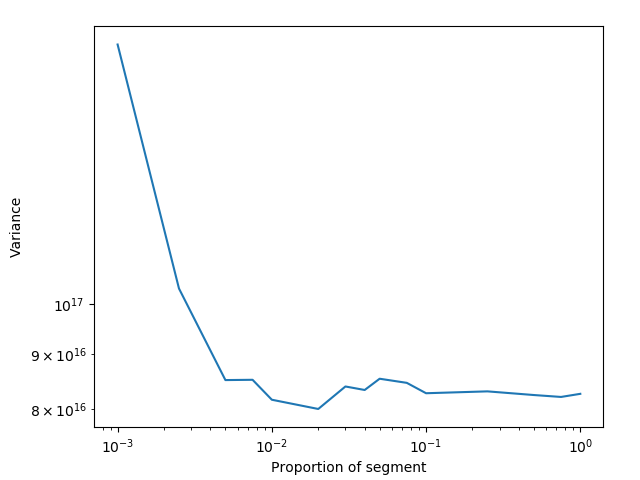
\includegraphics[width=1.45in]{Figure-3.2/Figure_3-AY336D.png}
    }
    \subfigure[AY272T]{
        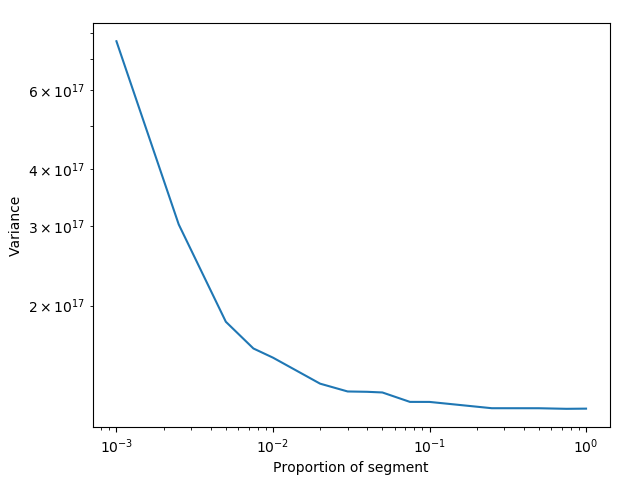
\includegraphics[width=1.45in]{Figure-3.2/Figure_3-AY272T.png}
    }
    
    \subfigure[AY306O]{
        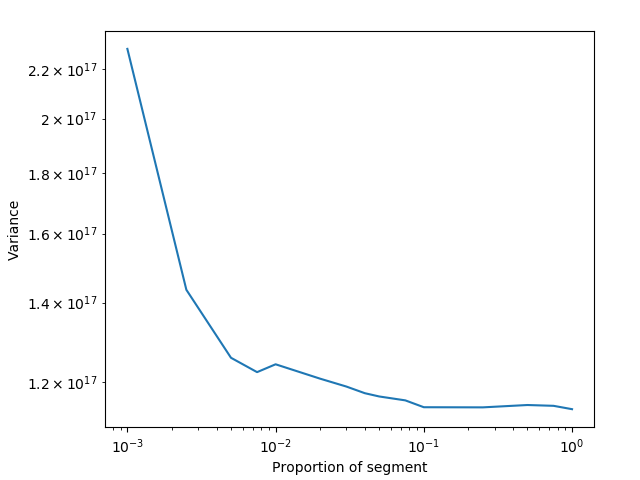
\includegraphics[width=1.45in]{Figure-3.2/Figure_3-AY306O.png}
    }
    \subfigure[AY251Z]{
        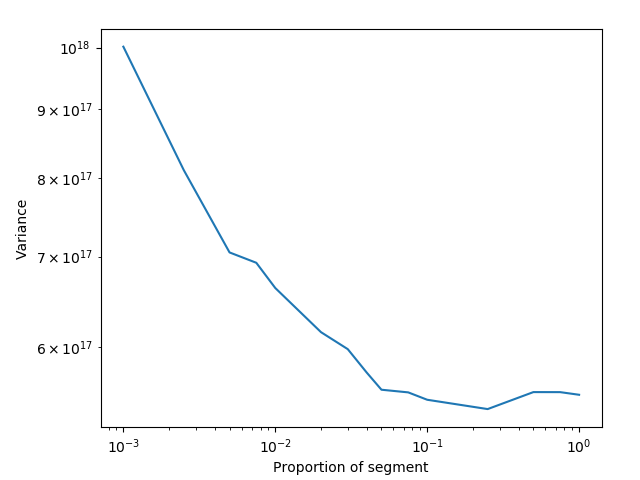
\includegraphics[width=1.45in]{Figure-3.2/Figure_3-AY251Z.png}
    }
    \centering
    \caption{Variance of Cluster with Different Schedule Proportion}
    \label{fig3.2-3}
\end{figure}

From the figure, we can learn that from the point of view of results, there is no significant difference between implementing greedy schedule for all the segments and for only 10\% of all segments. Few segments contributes most to the variance. Data from multiple clusters support this result.
